\subsection{随机试验}
\paragraph{}
\textbf{随机试验}的三个特点,用$E$表示:

\begin{enumerate}
  \item 可以在相同的条件下重复地进行
  \item 每次试验的可能结果不止一个,并且能事先明确试验的所有可能结果
  \item 进行一次试验之前不能确定哪一个结果会出现
\end{enumerate}

\paragraph{}
例子:

\label{s1_1}
\paragraph{}
$E_1$:抛一枚硬币,观察正面$H$、反面$T$出现的情况。

\subsection{样本空间、随机事件}
\subsubsection{样本空间}
\paragraph{}

随机试验$E$的所有可能结果组成的集合称为$E$的\textbf{样本空间},记为$S$,样本空间的元素,即每个结果,称为\textbf{样本点}。

\paragraph{}
例子,\linkref[s1_1]{$E_1$}的样本空间:

\paragraph{}
$S_1: \{H, T\};$

\subsubsection{随机事件}
\paragraph{}
试验$E$的样本空间$S$的子集为$E$的\textbf{随机事件},简称\textbf{事件},当且仅当这一子集中的一个样本点出现时,称这一\textbf{事件发生}。

\paragraph{}
由一个样本点组成的单点集,称为\textbf{基本事件},样本空间$S$包含所有的样本点,它是$S$自身的子集,在每次试验中它总是发生的,$S$称为\textbf{必然事件},空集$\varnothing$在每次试验中都不发生,称为\textbf{不可能事件}。

\subsubsection{事件间的关系与事件的运算}
\paragraph{}
事件是一个集合,符合集合的运算。

\paragraph{}
设试验$E$的样本空间为$S$,而$A, B, A_k(k = 1, 2, \cdots)$是$S$的子集:

\begin{enumerate}
  \item 若$A \subset B$,则事件$B$包含事件$A$,事件$A$发生必导致事件$B$发生。若$A \subset B$ 且 $B \subset A \Rightarrow A = B$,称事件$A$与事件$B$\textbf{相等}。
  \item 事件$A \cup B = \{x | x \in A \; \text{或} \; x \in B\}$称为事件$A$与事件$B$的\textbf{和事件}。${\displaystyle \bigcup_{k=1}^{n}} A_k$为$n$个事件$A_1, A_2, \cdots$的和事件。
  \item 事件$A \cap B=\{x | x \in A \; \text{且} \; x \in B\}$称为事件$A$与事件$B$的\textbf{积事件}。${\displaystyle \bigcap_{k=1}^{n}} A_k$为$n$个事件$A_1, A_2, \cdots$的积事件。
  \item 事件$A-B=\{x | x \in A \; \text{且} \; x \notin B\}$称为事件$A$与事件$B$的\textbf{差事件}。
  \item 若 $A \cap B = \varnothing$,且称事件$A$与$B$是\textbf{互不相容的},或\textbf{互斥的}。
  \item 若 $A \cup B = S$ 且 $A \cap B = \varnothing$,称事件$A$与事件$B$互为\textbf{逆事件},又称\textbf{对立事件},记为$\overline{A} = S - A$。
\end{enumerate}

\paragraph{}
集合中,有些教材,\textbf{差运算}$S - A$用$S \symbol{92} A$表示,\textbf{补集}$\overline{A}$用$A^{c}$表示。

\begin{figure}[h]
\centering
  %------- 第1行 -------
  \begin{subfigure}[t]{0.3\linewidth}
    \centering
      % A 包含于 B
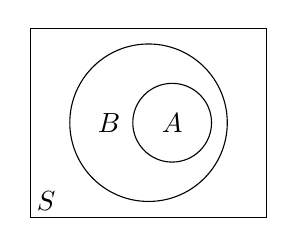
\begin{tikzpicture}
  %---------------- subset ----------------
  \draw (0.3,0) circle [radius=.5];
  \node at (0.3,0) {$A$};

  \draw (0,0) circle [radius=1];
  \node at (-0.5,0) {$B$};

  \draw (-1.5,-1.2) rectangle (1.5,1.2);
  \node at (-1.3,-1) {$S$};
\end{tikzpicture}

      \caption{$A \subset B$}
      \label{1_A_subset_B}
  \end{subfigure}
  \begin{subfigure}[t]{0.3\linewidth}
    \centering
      % A 并 B
\begin{tikzpicture}
  %---------------- cup ----------------
  \draw (-0.8,0) circle [radius=.5];
  \fill[pattern=north west lines] (-0.8,0) circle [radius=.5];
  \node[fill=white, inner sep=.5] at (-.95,0) {$A$};

  \draw (0.3,0) circle [radius=1];
  \fill[pattern=north west lines] (0.3,0) circle [radius=1];
  \node[fill=white, inner sep=.5] at (0.3,0) {$B$};

  \draw (-1.5,-1.2) rectangle (1.5,1.2);
  \node at (-1.3,-1) {$S$};
\end{tikzpicture}

      \caption{$A \cup B$}
      \label{1_A_cup_B}
  \end{subfigure}
  \begin{subfigure}[t]{0.3\linewidth}
    \centering
      % A 交 B
\begin{tikzpicture}
  % circle A
  \draw (-.8,0) circle [radius=.5];
  \node at (-.95,0) {$A$};
  % circle B
  \draw (0.3,0) circle [radius=1];
  \node at (0.3,0) {$B$};
  % A 交 B
  \begin{scope}
    \clip (-.8, 0) circle (.5);
    \clip (0.3, 0) circle (1);
    \fill[pattern=north west lines] (-0.7,-1) rectangle (1.3,1);
  \end{scope}
  % rectangle S
  \draw (-1.5,-1.2) rectangle (1.5,1.2);
  \node at (-1.3,-1) {$S$};
\end{tikzpicture}

      \caption{$A \cap B$}
      \label{1_A_cap_B}
  \end{subfigure}

  \bigskip %------- 第2行 -------
  \begin{subfigure}[b]{0.3\linewidth}
    \centering
      % A - B
\begin{tikzpicture}
  % 阴影部分
  \fill[pattern=north west lines] (-.8,0) circle [radius=.5];
  % circle B
  \draw[fill=white] (0.3,0) circle [radius=1];
  \node at (0.3,0) {$B$};

  % circle A
  \draw (-.8,0) circle [radius=.5];
  \node[fill=white, inner sep=.5] at (-.95,0) {$A$};

  \draw (-1.5,-1.2) rectangle (1.5,1.2);
  \node at (-1.3,-1) {$S$};
\end{tikzpicture}

      \caption{$A - B$}
      \label{1_A_diffence_B}
  \end{subfigure}
  \begin{subfigure}[b]{0.3\linewidth}
    \centering
      % A 交 B = 空集
\begin{tikzpicture}

  % circle B
  \draw[pattern=north west lines] (-.45,.15) circle [radius=1];
  \node[fill=white, inner sep=.5] at (-.45,.15) {$B$};

  % circle A
  \draw[pattern=north west lines] (.95,-.65) circle [radius=.5];
  \node[fill=white, inner sep=.5] at (.95,-.65) {$A$};

  \draw (-1.5,-1.2) rectangle (1.5,1.2);
  \node at (-1.3,-1) {$S$};
\end{tikzpicture}

      \caption{$A \cap B = \varnothing$}
      \label{1_A_cap_nothing_B}
  \end{subfigure}
  \begin{subfigure}[b]{0.3\linewidth}
    \centering
      % B的补集
\begin{tikzpicture}
  % 基本集 S
  \draw[pattern=north west lines] (-1.5,-1.2) rectangle (1.5,1.2);
  \node[fill=white, inner sep=.5] at (-1.3,-1) {$S$};

  % circle B
  \draw[fill=white] (0.3,0) circle [radius=1];
  \node at (0.3,0) {$B$};
  \node[fill=white, inner sep=.5] at (-.95,0) {$\overline{B}$};
\end{tikzpicture}

      \caption{$B \cup \overline{B} = S; B \cap \overline{B} = \varnothing$}
      \label{1_B_complement}
  \end{subfigure}
  \caption{事件$A$和事件$B$的关系和运算}
  \label{事件A和事件B的关系和运算}
\end{figure}

\subsubsection{常用运算公式}
\paragraph{}
设$A, B, C$为事件,则:

\begin{enumerate}
  \item 交换律:
  \begin{align}
    \begin{split}
    A \cup B = B \cup A; \\
    A \cap B = B \cap A
    \end{split}
  \end{align}
  \item 结合律:
  \begin{align}
    \begin{split}
    A \cup (B \cup C) = (A \cup B) \cup C; \\
    A \cap (B \cap C) = (A \cap B) \cap C
    \end{split}
  \end{align}
  \item 分配律:
  \begin{align}
    \begin{split}
    A \cup (B \cap C) = (A \cup B) \cap (A \cup C); \\
    A \cap (B \cup C) = (A \cap B) \cup (A \cap C)
    \end{split}
  \end{align}
  \item 德摩根律:
  \begin{align}
    \begin{split}
    \overline{A \cup B} = \overline{A} \cap \overline{B}; \\
    \overline{A \cap B} = \overline{A} \cup \overline{B}
    \end{split}
  \end{align}
\end{enumerate}

\subsection{频率与概率}
\subsubsection{频率}
\paragraph{}
\textbf{定义\;}在相同的条件下,进行了$n$次试验,在这$n$次试验中,事件$A$发生的次数$n_A$称为事件$A$发生的\textbf{频数}。比值$n_A / n$称为事件$A$发生的\textbf{频率},记为$f_n(A)$。

\paragraph{}
频率具有下述基本性质:
\begin{enumerate}
  \item $0 \leq f_n(A) \leq 1$
  \item $f_n (S) = 1$
  \item 若$A_1, A_2, \cdots, A_k$是两两互不相容的事件,则
  \begin{equation}
    f_n(A_1 \cup A_2 \cup \cdots \cup A_k) = f_n(A_1) + f_n(A_2) + \cdots + f_n(A_k)
  \end{equation}
\end{enumerate}

\paragraph{}
需要重复大量试验,频率$f_n(A)$呈现稳定性,稳定于某个常数。这种稳定性称为\textbf{统计规律性}。重复大量次数试验,计算频率$f_n(A)$,以它表征事件$A$发生可能性的大小是合适的。

\paragraph{}
实际中,不可能每个事件都可以做大量的试验,因此理论研究通过\textbf{概率}来表征事件发生可能性大小。

\subsubsection{概率}
\paragraph{}
\textbf{定义\;}设$E$是随机试验,$S$是它的样本空间,对于$E$的每一个事件$A$赋予一个实数,记为$P(A)$,称为事件$A$的\textbf{概率},如果集合函数$P(\cdot)$满足:
\begin{enumerate}
  \item \textbf{非负性:}对于每一个事件$A$,有$P(A) \geq 0$
  \item \textbf{规范性:}对于必然事件$S$,有$P(S)=1$
  \item \textbf{可列可加性:}设$A_1, A_2, \cdots$是两两互不相容的事件,即对于$A_iA_j=\varnothing, i \neq j, i, j=1,2,\cdots,$有$ P(A_1 \cup A_2 \cup \cdots)=P(A_1)+P(A_2)+\cdots$
\end{enumerate}

\paragraph{}
推导性质:

\begin{enumerate}
  \item $P(\varnothing) = 0$
  \item \textbf{有限可加性\;}若$A_1, A_2, \cdots, A_n$是两两互不相容的事件,则有$ P(A_1 \cup A_2 \cup \cdots \cup A_n)=P(A_1)+P(A_2)+\cdots+P(A_n)$
  \item 设$A, B$是两个事件,若$A \subset B$,则有:
  \begin{align}
    \begin{split}
    P(B-A) =&\; P(B) - P(A); \\
    P(B) \geq &\; P(A)
    \end{split}
  \end{align}
  \item 对于任一事件$A$,$P(A) \leq = 1$
  \item \textbf{逆事件的概率\;}对于任一事件$A$,有$P(\overline{A}) = 1-P(A)$
  \item \textbf{加法公式\;}对于任意两个事件$A, B$有$P(A \cup B)=P(A)+P(B)-P(AB)$,\\ 一般,对于任意$n$个事件$A_1, A_2, \cdots , A_n$,可用归纳法证得
  \begin{align}
    \begin{split}
    P(A_1 \cup A_2 \cup \cdots \cup A_n) =& \; \sum_{i=1}^{n}P(A_i) - \sum_{1 \leq i < j \leq n}P(A_iA_j) \\
    & \; + \sum_{1 \leq i < j < k \leq n}P(A_iA_jA_k)+ \cdots + (-1)^{n-1}P(A_1A_2 \cdots A_n)
    \end{split}
  \end{align}
\end{enumerate}

\subsection{等可能概型(古典概型)}
\paragraph{}
\textbf{等可能概型\;}的特点:
\begin{enumerate}
  \item 试验的样本空间只包含有限个元素
  \item 试验中每个基本事件发生的可能性相同
\end{enumerate}
\paragraph{}
若事件$A$包含$k$个基本事件,即$A = \{e_{i_1}\} \cup \{e_{i_2}\} \cup \cdots \cup \{e_{i_k}\}$,这里$i_1, i_2, \cdots, i_k$是$1, 2, \cdots, n$中某$k$个不同的数,则:
\begin{equation}
  P(A) = \sum_{j=1}^{k}P(\{e_{i_j}\}) = \frac{k}{n} = \frac{\text{$A$包含的基本事件数}}{\text{$S$中基本事件的总数}}
\end{equation}

\paragraph{}
概率很小的事件在一次试验中实际上几乎是不发生的,称为\textbf{实际推断原理}。
\paragraph{}
\textbf{例\;}某接待站在某一周曾接待过$12$次来访,已知所有这$12$次接待都是在周二和周四进行的,问是否可以推断接待时间是有规定的?
\paragraph{}
\textbf{解\;}假设接待站的接待时间没有规定,而各来访者在一周的任意一天中去接待站是等可能的,那么,$12$次接待来访者都在周二、周四的概率为
\begin{equation*}
  \frac{2^{12}}{7^{12}} = 0.000 \; 000 \; 3
\end{equation*}
\paragraph{}
因此,推断出接待时间是有规定的。

\subsection{条件概率}
\subsubsection{条件概率}
\paragraph{}
\label{条件概率定义}
\textbf{定义\;}设试验的基本事件总数为$n, A$所包含的基本事件数为$m(m>0)$,$AB$所包含的基本事件数为$k$,即:
\begin{equation}
  P(B|A) = \frac{k}{m} = \frac{k/n}{m/n} = \frac{P(AB)}{P(A)},
\end{equation}
称为在事件$A$发生的条件下事件$B$发生的\textbf{条件概率}。
\paragraph{}
条件概率$P(\cdot | A)$符合概率定义中的三个条件:
\begin{enumerate}
  \item \textbf{非负性:}对于每一事件$B$,有$P(B|A)\geq 0$
  \item \textbf{规范性:}对于必然事件$S$,有$P(S|A)=1$
  \item \textbf{可列可加性:}设$B_1, B_2, \cdots$是两两互不相容的事件,则:
  \begin{equation}
    P(\bigcup_{i=1}^\infty B_i | A) = \sum_{i=1}^\infty P(B_i | A),
  \end{equation}
\end{enumerate}
对任意事件$B_1, B_2$有$P(B_1 \cup B_2 | A) = P(B_1 | A) + P(B_2 | A) - P(B_1B_2|A)$

\subsubsection{乘法定理}
\paragraph{}
由\linkref[条件概率定义]{条件概率的定义},可得到下述定理。
\paragraph{}
\textbf{乘法定理\;}设$P(A)>0$,则有
\begin{equation}
  \label{乘法公式}
  P(AB) = P(B|A)P(A)
\end{equation}
\eqref{乘法公式}式称为\textbf{乘法公式}。
\paragraph{}
一般,设$A_1, A_2, \cdots, A_n$为$n$个事件,$n \geq 2$,且$P(A_1A_2\cdots A_{n-1}) > 0$,则有:
\begin{equation}
  P(A_1A_2\cdots A_n) = P(A_n|A_1A_2\cdots A_{n-1})P(A_{n-1}|A_1A_2\cdots A_{n-2})\cdots P(A_2|A_1)P(A_1).
\end{equation}

\subsubsection{全概率公式和贝叶斯公式}
\paragraph{}
\textbf{定义\;}设$S$为试验$E$的样本空间,$B_1, B_2, \cdots, B_n$为$E$的一组事件,若:
\begin{enumerate}
  \item $B_iB_j=\varnothing, i \neq j, i,j = 1,2,\cdots,n$
  \item $B_1 \cup B_2 \cup \cdots \cup B_n = S$
\end{enumerate}
则称$B_1,B_2,\cdots,B_n$为样本空间$S$的一个\textbf{划分}。若$B_1,B_2,\cdots,B_n$是样本空间的一个划分,那么,对每次试验,事件$B_1,B_2,\cdots,B_n$中必有一个且仅有一个发生。

\paragraph{}
\textbf{定理\;}设试验$E$的样本空间为$S$,$A$为$E$的事件,$B_1,B_2,\cdots,B_n$为$S$的一个划分,且$P(B_i)>0(i=1,2,\cdots,n)$,则:
\begin{align}
  \label{全概率公式}
  \begin{split}
    P(A) =&\; P(A|B_1)P(B_1) + P(A|B_2)P(B_2)+ \cdots + \\
    &\; P(A|B_n)P(B_n).
  \end{split}
\end{align}
\eqref{全概率公式}式称为\textbf{全概率公式}。

\paragraph{}
\textbf{定理\;}设试验$E$的样本空间为$S$,$A$为$E$的事件,$B_1,B_2,\cdots,B_n$为$S$的一个划分,且$P(A)>0, P(B_i)>0(i=1,2,\cdots,n)$,则:
\begin{equation}
  \label{贝叶斯公式}
  P(B_i |A) = \frac{P(B_iA)}{P(A)} = \frac{P(A|B_i)P(B_i)}{\displaystyle \sum_{j=1}^n P(A|B_j)P(B_j)}, i = 1,2,\cdots,n.
\end{equation}
\eqref{贝叶斯公式}式称为\textbf{贝叶斯(Bayes)公式}。

\paragraph{}
由以往的数据分析得到的,叫做\textbf{先验概率}。得到信息后再重新加以修正的概率叫做\textbf{后验概率}

\subsection{独立性}
\paragraph{}
设$A,B$是试验$E$的两事件,若$P(A)>0$,可以定义$P(B|A)$。一般,$A$的发生对$B$发生的概率是有影响的,这时$P(B|A) \neq P(B)$,只有在这种影响不存在时才会有$P(B|A)=P(B)$,这时有:
\begin{equation}
  P(AB) = P(B|A)P(A) = P(A)P(B)
\end{equation}
如果满足上式,则称事件$A,B$\textbf{相互独立},简称$A,B$\textbf{独立}。

\paragraph{}
\textbf{定理一\;}设$A,B$是两事件,且$P(A)>0$,若$A,B$相互独立,则$P(B|A)=P(B)$,反之亦然。

\paragraph{}
\textbf{定理二\;}若事件$A$与$B$相互独立,则下列各对事件也相互独立:$A$与$\overline{B}$,$\overline{A}$与$B$,$\overline{A}$与$\overline{B}$。

\paragraph{}
\textbf{定义\;}设$A,B,C$是三个事件,如果满足等式:
\begin{equation}
  \left. \begin{array}{rcl}
    P(AB) & = & P(A)P(B), \\
    P(BC) & = & P(B)P(C), \\
    P(AC) & = & P(A)P(C), \\
    P(ABC) & = & P(A)P(B)P(C),
  \end{array} \right\}
\end{equation}
则称事件$A,B,C$\textbf{相互独立}

\paragraph{}
一般,设$A_1,A_2,\cdots,A_n$是$n(n \geq 2)$个事件,如果对于其中任意$2$个,任意$3$个,$\cdots$,任意$n$个事件的积事件的概率,都等于各事件概率之积,则称事件$A_1,A_2,\cdots,A_n$\textbf{相互独立}。

\paragraph{}
\textbf{推论\;}若事件$A_1,A_2,\cdots,A_n(n \geq 2)$相互独立,则其中任意$k(2 \leq k \leq n)$个事件也是相互独立的。

\paragraph{}
\textbf{推论\;}若$n$个事件$A_1,A_2,\cdots,A_n(n \geq 2)$相互独立,则将$A_1,A_2,\cdots,A_n$中任意多个事件换成它们各自的对立事件,所得的$n$个事件仍相互独立。
